\chapter{Robot}
    The robot we simulate and use is based on the multistable joint we have seen on section \ref{sec:multistable}. In fact each leg is a multistable joint. As we have different sequences for each leg, the motion of the robot is hard to predict. We will first go through the structure of the robot before talking about the actuation of the legs. Then we will cover how the legs are articulated and how they are touching the ground. 
    
    \begin{figure}[h!]
        \centering
        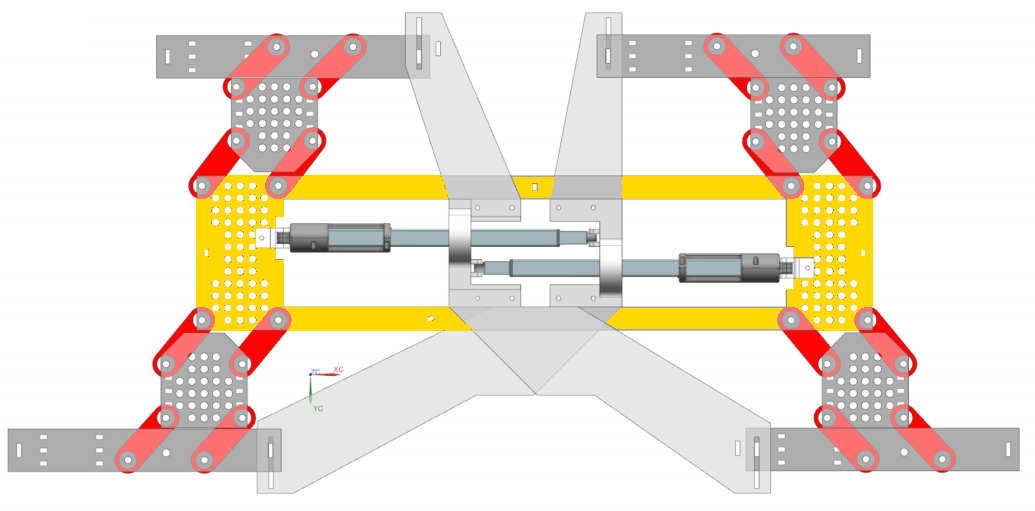
\includegraphics[width=0.8\textwidth]{images/top_view_robot.png}
        \caption{Top view of the robot. We can see four identical multistable joint that act as legs. The yellow part is the main frame. This main frame is connecting the ground block of the four multistable joint together. }
        \label{fig:robot_top_view}
    \end{figure}
    
    \section{Structure}
        Let's dive into the structure of the robot, Figure \ref{fig:robot_top_view} shows a top view of the structure of the robot. Each multistable structure also consists of three blocks linked by red arms. We can recognize four multistable structures in the robot. The main frame is the yellow part of the robot, it links the bottom block of all multistable structures together, this means that the position of the four bottom blocks are static relative to each other. 
        
        
        The end points of the legs are attached to the middle and the top block of each multistable mechanism. The way they move will be described the section \ref{sec:legs}. Two actuators are attached to the main yellow frame, each actuators controls two multistable joint and they are oriented in a $180°$ shape, being co-linear but facing opposite direction. 
        
        
        \begin{figure}[h!]
            \centering
            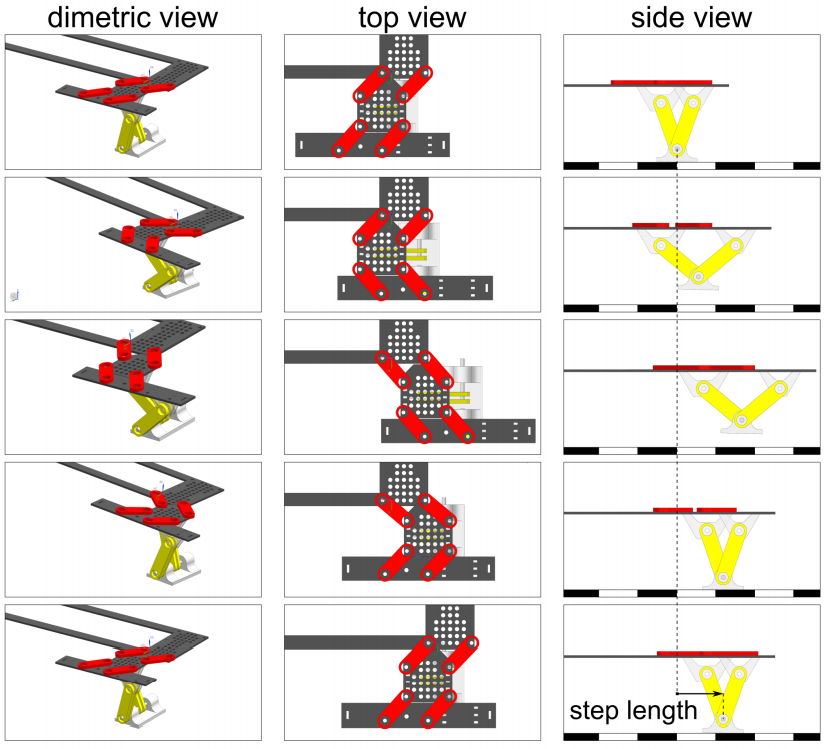
\includegraphics[width=0.8\textwidth]{images/forward_step.png}
            \caption{Specific focus on a leg of a robot, here specifically in sequence B, where the top block is moving before the middle block. The leg is attached to a multistable structure and consists of a two arms linking the top block to the middle block with a common joint. We can see three views in the sequence order, the first columns is a dimetric view of the leg, where we can have a 3D view of the cycle. The second columns represent a top view of the leg that shows how the blocks are moving in the sequence order, where the top block is always moving before the middle block. Finally, the third columns is a side view of the leg with the two arms and the end plate. We can see how the legs is moving horizontally and vertically. We also see that it performs a cycle that is represented by a hysteresis.}
            \label{fig:forward_step}
        \end{figure}
        
    \section{Legs}\label{sec:legs}
        Legs are connected directly to a multistable joint system. They are right underneath the middle and the top block of the joint. We can see on Figure \ref{fig:forward_step} a side view, a top view and a dimetric view of a the legs during a forward step. 
        The leg is build with two arms that are connected together on one end and the second end is respectively connected to the middle block and the top block. This forms a triangular shape as we can see on the side view of Figure \ref{fig:forward_step}. The position of the end of the leg in contact with the ground will be affected by the positions of the middle and the top block. The distance between the two blocks will affect the heights of the end of the leg. We can see during the forward step that when both middle and top blocks moves to a side at the same pace (bottom joint is moving), the end of the leg is moving at the same pace. On the other hand, when the top joint is moving, the only block that is moving is the top block, therefore it will affect a bit the horizontal position of the end of the leg, but it will especially change the height of the leg. When the distance between the two blocks are increasing, the height is decreasing. When the distance is decreasing, the height is increasing. We can already see here that due to the different sequence, the leg motion is drawing a hysteresis. This hysteresis is important as it allows the robot to move in different directions depending of the actuation and the sequences selected for the legs. 
        
    \section{Actuation}\label{sec:actuation}
        The actuation is performed with linear actuators that are connected to the legs in a specific way. First we can see on Figure \ref{fig:robot_top_view} that they are oriented in the same axis but they are facing opposite direction. They are actuated separately and we will define a phase difference of $0°$ when when both actuators extends and retract at the same time and at the same speed. A phase difference of $180°$ will occurs when one actuator is extending while the other is retracting. As we have two actuators and four legs to connect, we need to associate them in pair, each actuator will be connected to a pair of legs that are in diagonal in the robot view. As seen on Figure \ref{fig:legs_connection}, we have two groups of legs, the green group includes legs 1 and 4 and is linked to the first actuator. The second group is the magenta group and includes legs 2 and 3 that are linked to the second actuator. 
        
        \begin{figure}
            \centering
            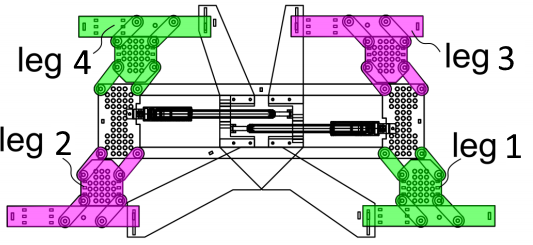
\includegraphics[width=0.5\textwidth]{images/legs_connection.png}
            \caption{Legs connection to actuators, we can see two groups of colors, green groups consists of legs 1 and legs 4 are connected to one actuator. This means that the top block of each multistable joint will move in coordination with the actuator in the horizontal axis. The second group consists of magenta blocks (legs 2 and legs 3) and is linked to the second actuator.}
            \label{fig:legs_connection}
        \end{figure}